
%----------------------------------------------------------------------------------------
%	Lecture 1
%----------------------------------------------------------------------------------------

\chapter{The Need for Quantum Mechanics}

\bigbreak
\section{State of the Universe}

Three unexplained experiments :
\begin{enumerate}
	\item Blackbody Spectrum
	\item Photoelectric Effect
	\item Bright Line Spectra
\end{enumerate}

\subsection{Blackbody Spectrum}
Certain objects are called blackbodies because the emit electromagnetic radiation of all wavelengths. The sun is an example of a blackbody.

The diagram below shows the intensity of light emitted by a blackbody of a certain wavelength by atoms at a certain temperature.
But the prediction of classical mechanics is much different than the actual data.

\begin{figure}[ht!]
	\centering
	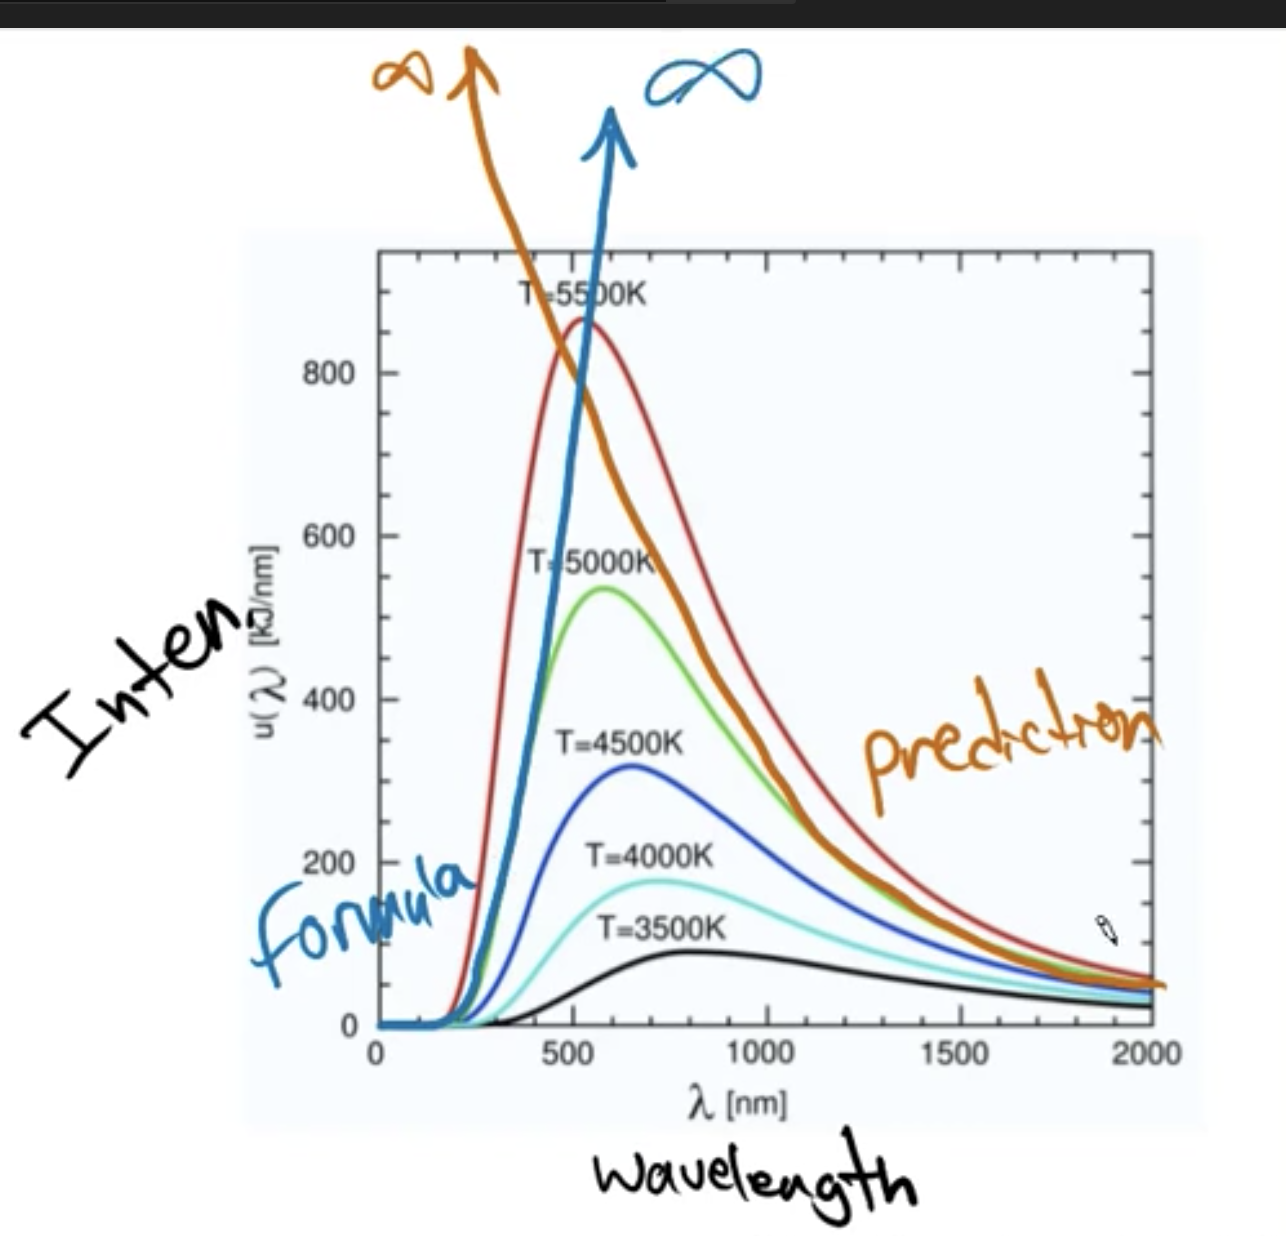
\includegraphics[scale=0.5]{./images/lecture_1_figure_1.png}
	\caption{Intensity of Light Emitted of a certain wavelength}
\end{figure}

Here we have a prediction that predicts infinite intensity of light emitted.
And on another hand, we have a formula that fits the lower end of the data but also goes to infinty at large wavelengths.

\pagebreak


\subsection{Photoelectric Effect}

In this experiment, we have light coming in which exites the electrons the material to leave the atom. We recieve the electrons in the opposite side of the setup and count them.
We then apply a certain opposing voltage to the setup to stop the electrons. But if the electrons have enough energy then they will cross this voltage anyway.
So we increase the voltage until no electrons can cross the voltage and we call that voltage $V_{stop}$ or stopping voltage.

\begin{figure}[ht!]
	\centering
	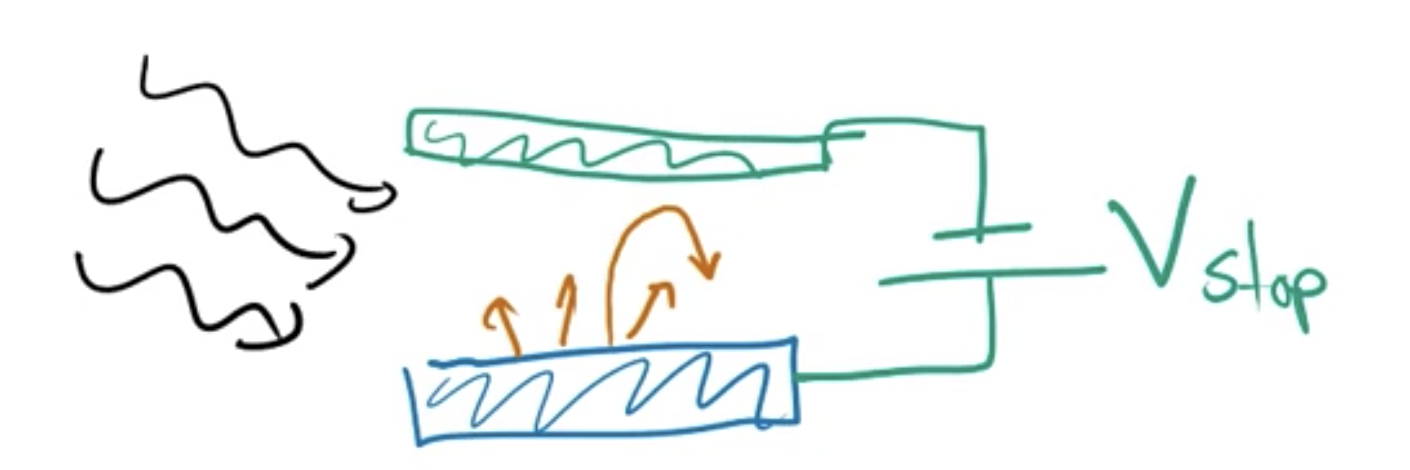
\includegraphics[scale=0.5]{./images/lecture_1_figure_2.png}
	\caption{The Setup For Photoelectric Effect}
\end{figure}

The Classical Electromagnetism tells us that light is an electromagnetic wave.
So if we increase the intensity of the incoming light, then the magnitude of the electric field will increase 
so the energy of the escaping electrons will increase and the stopping voltage will increase as well.

Another parameter of the incoming light is its frequency. 
If we increase the frequency, we don't necessarily have more intense light.
So the electric field is also the same. Thus, the energy and the stopping voltage are also the same.

But in reality, something completely different happens.
When we increase the intensity, the stopping voltage stays the same.
But when we increase the frequency, the stopping voltage increases.

\begin{figure}[ht!]
	\centering
	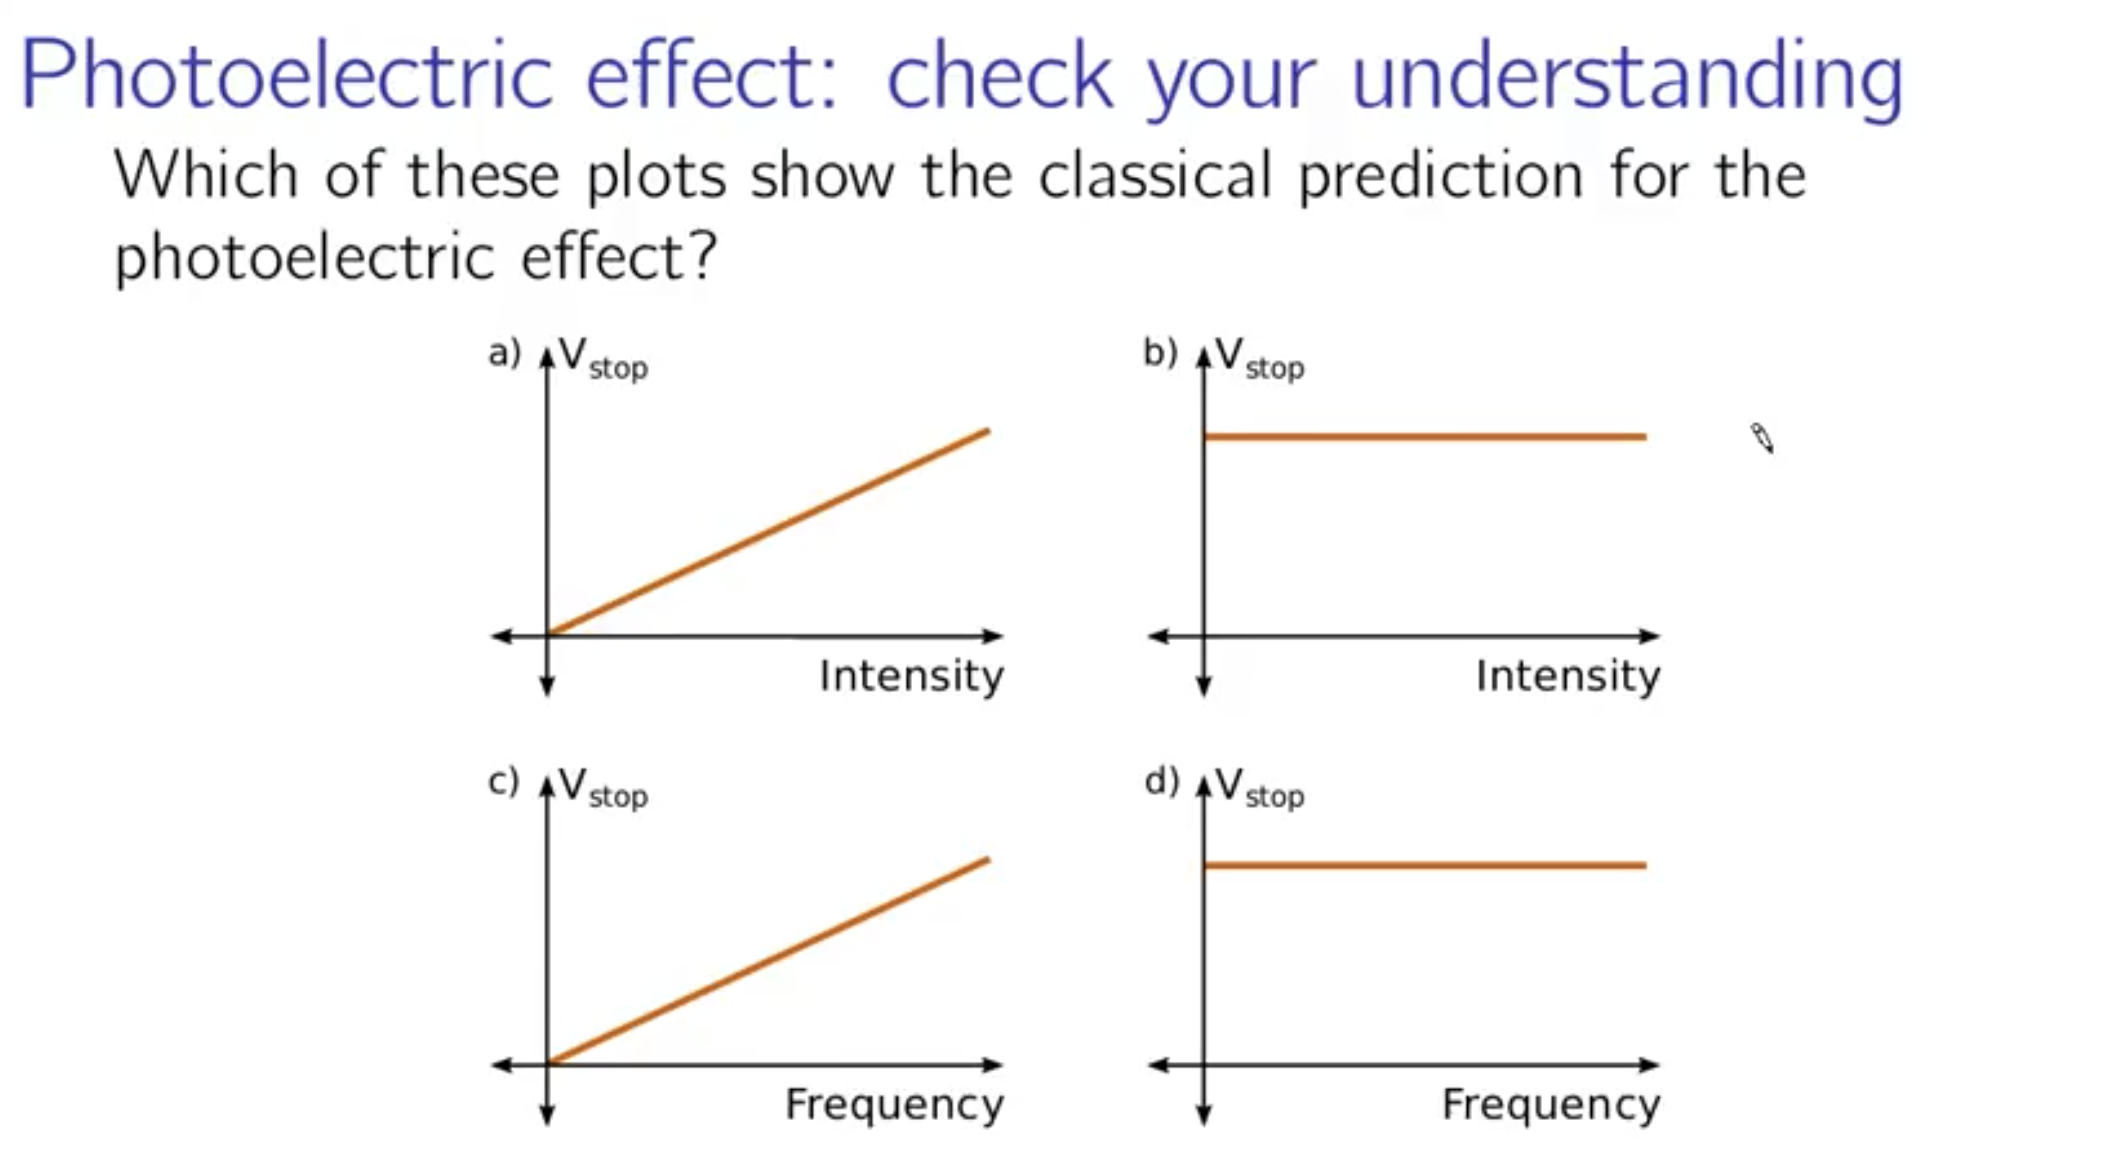
\includegraphics[scale=0.3]{./images/lecture_1_figure_3.png}
	\caption{Quiz : Plot of Stopping Voltage}
\end{figure}

The Classical Electromagnetism predicts (a) and (d) but in reality we get (b) and (c).

\pagebreak

\subsection{Bright Line Spectra}

The third experiment is Bright Line Spectra. 
If you heat up a substance then that will emit light.
In this case the spectrum of light looks like the following.

\begin{figure}[ht!]
	\centering
	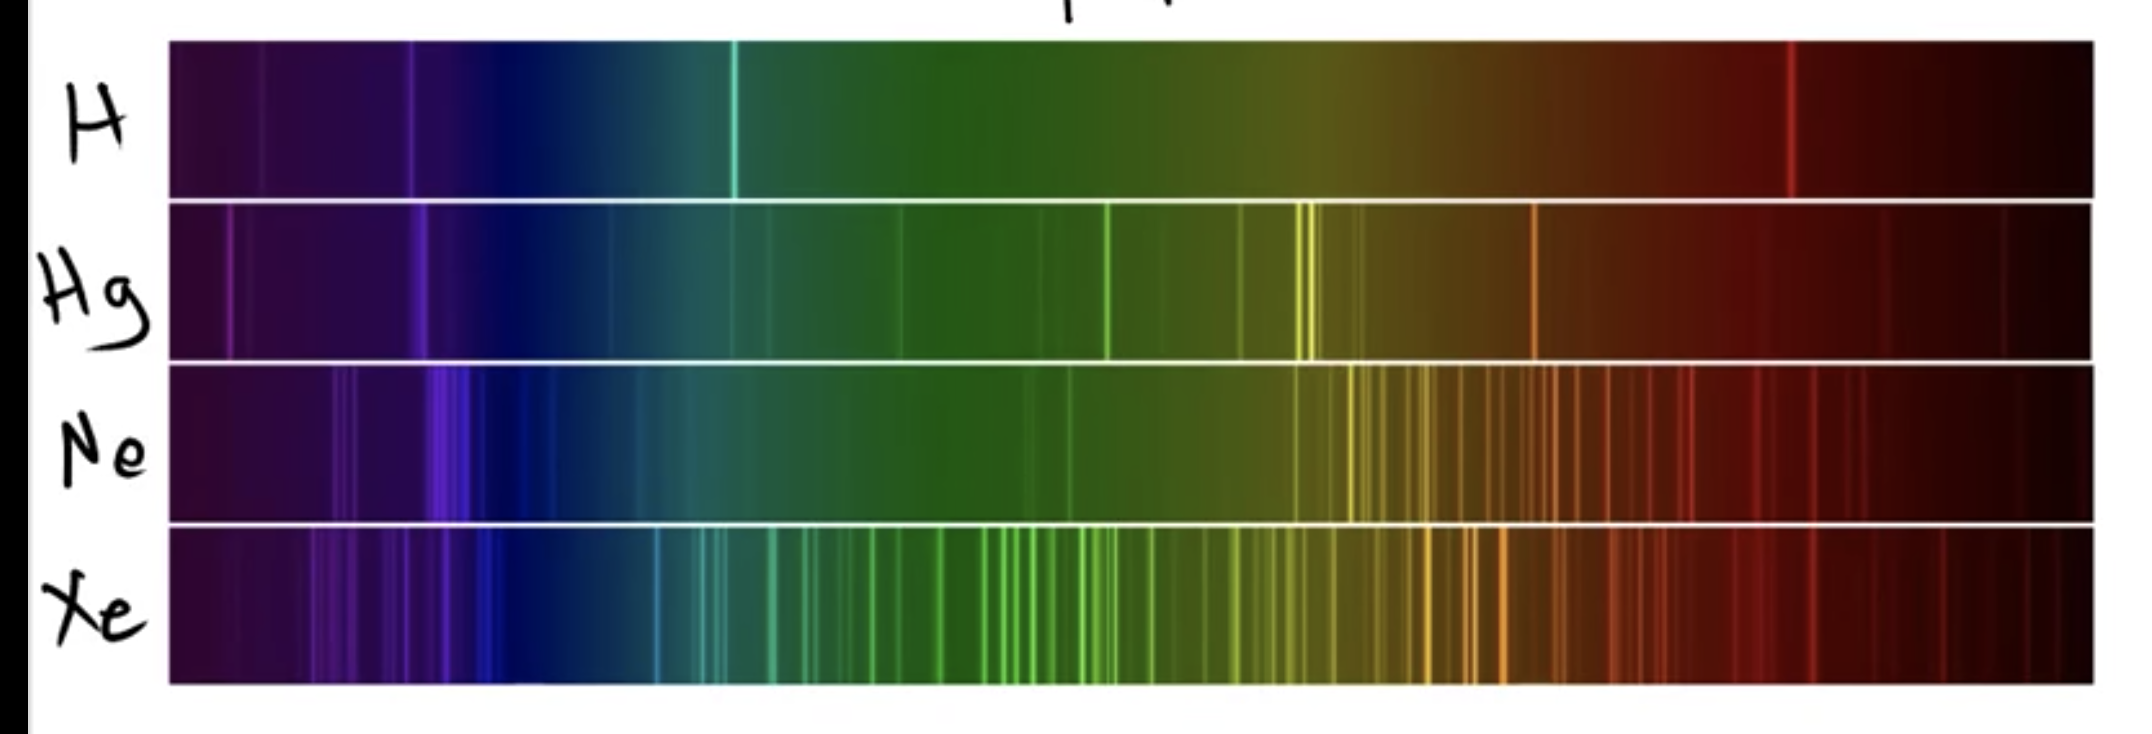
\includegraphics[scale=0.3]{./images/lecture_1_figure_4.png}
	\caption{Bright Line Spectra}
\end{figure}

The classical electromagnetism predicts a continuous distribution.
That is, every frequency of light will be emitted in some amount by those atoms.

\subsection{Solution}

The solution to the blackbody spectrum problems was divised by Max Planck.
He said that the light is not a continuous wave but it comes in discrete chunks. 
And it is aborbed and emitted in those discrete chunks only.
He said that the energy of a light chunk can be $E = n \hbar f$ where $\hbar$ is the Planck's constant, 
$f$ is the frequency of light and  $n$ is an integer.

$$ \hbar = 6.626 \times 10^{-34} J s $$


This was just an mathematical patch for electromagnetism at first but as time passed other
scientists made thoeries and those theories made prediction that were verified later.